
\section{C4 Modeling}

First of all for the sake of simplicity and understanding the design will be explained using the C4 model architecture. 

As shown in the Figure \ref{fig:c41}, a System Context diagram is shown and it allows to step back and see the big picture of the application.

\begin{figure}[h!]
    \centering
    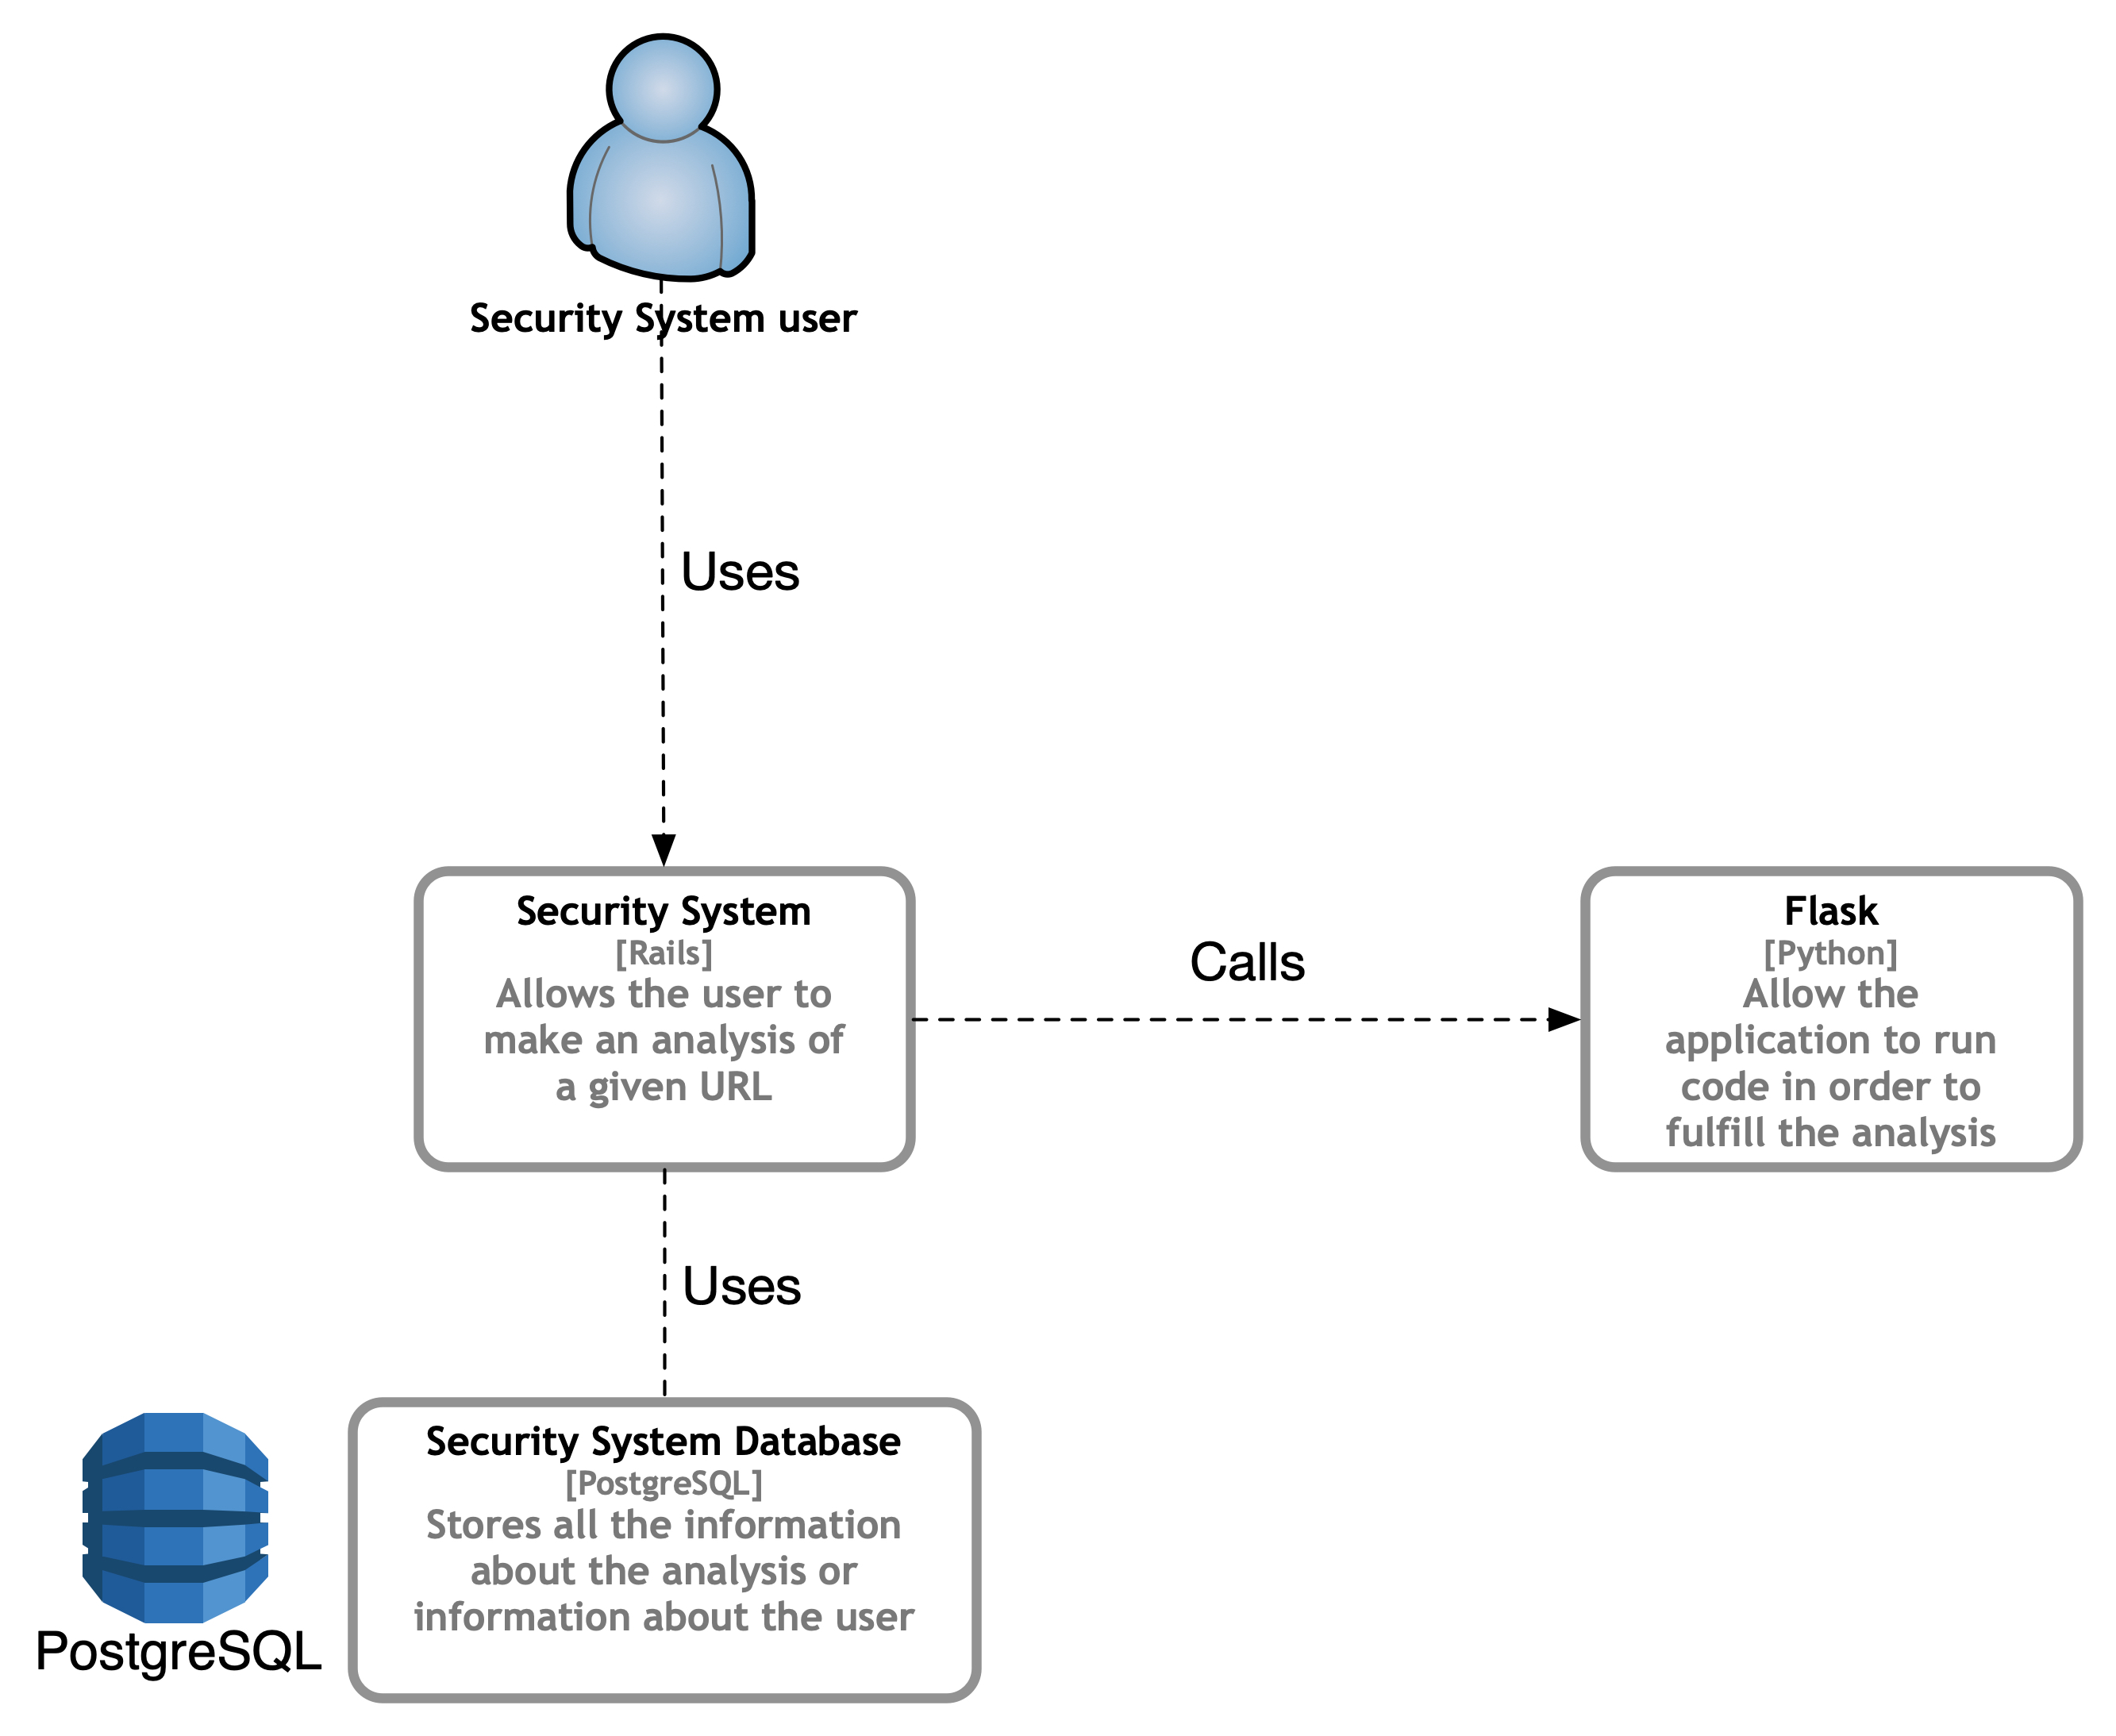
\includegraphics[width=10cm]{img/C41.jpg}
    \caption{System Context diagram}
    \label{fig:c41}
\end{figure}

\clearpage

In the Figure \ref{fig:c42} the Container Diagram helps explaining the system in a deeper overview than the System Context Diagram. The Container diagram shows the high-level shape of the software architecture and how responsibilities are distributed across it. It also shows the major technology choices and how the containers communicate with one another \cite{c4model}.

\begin{figure}[h!]
    \centering
    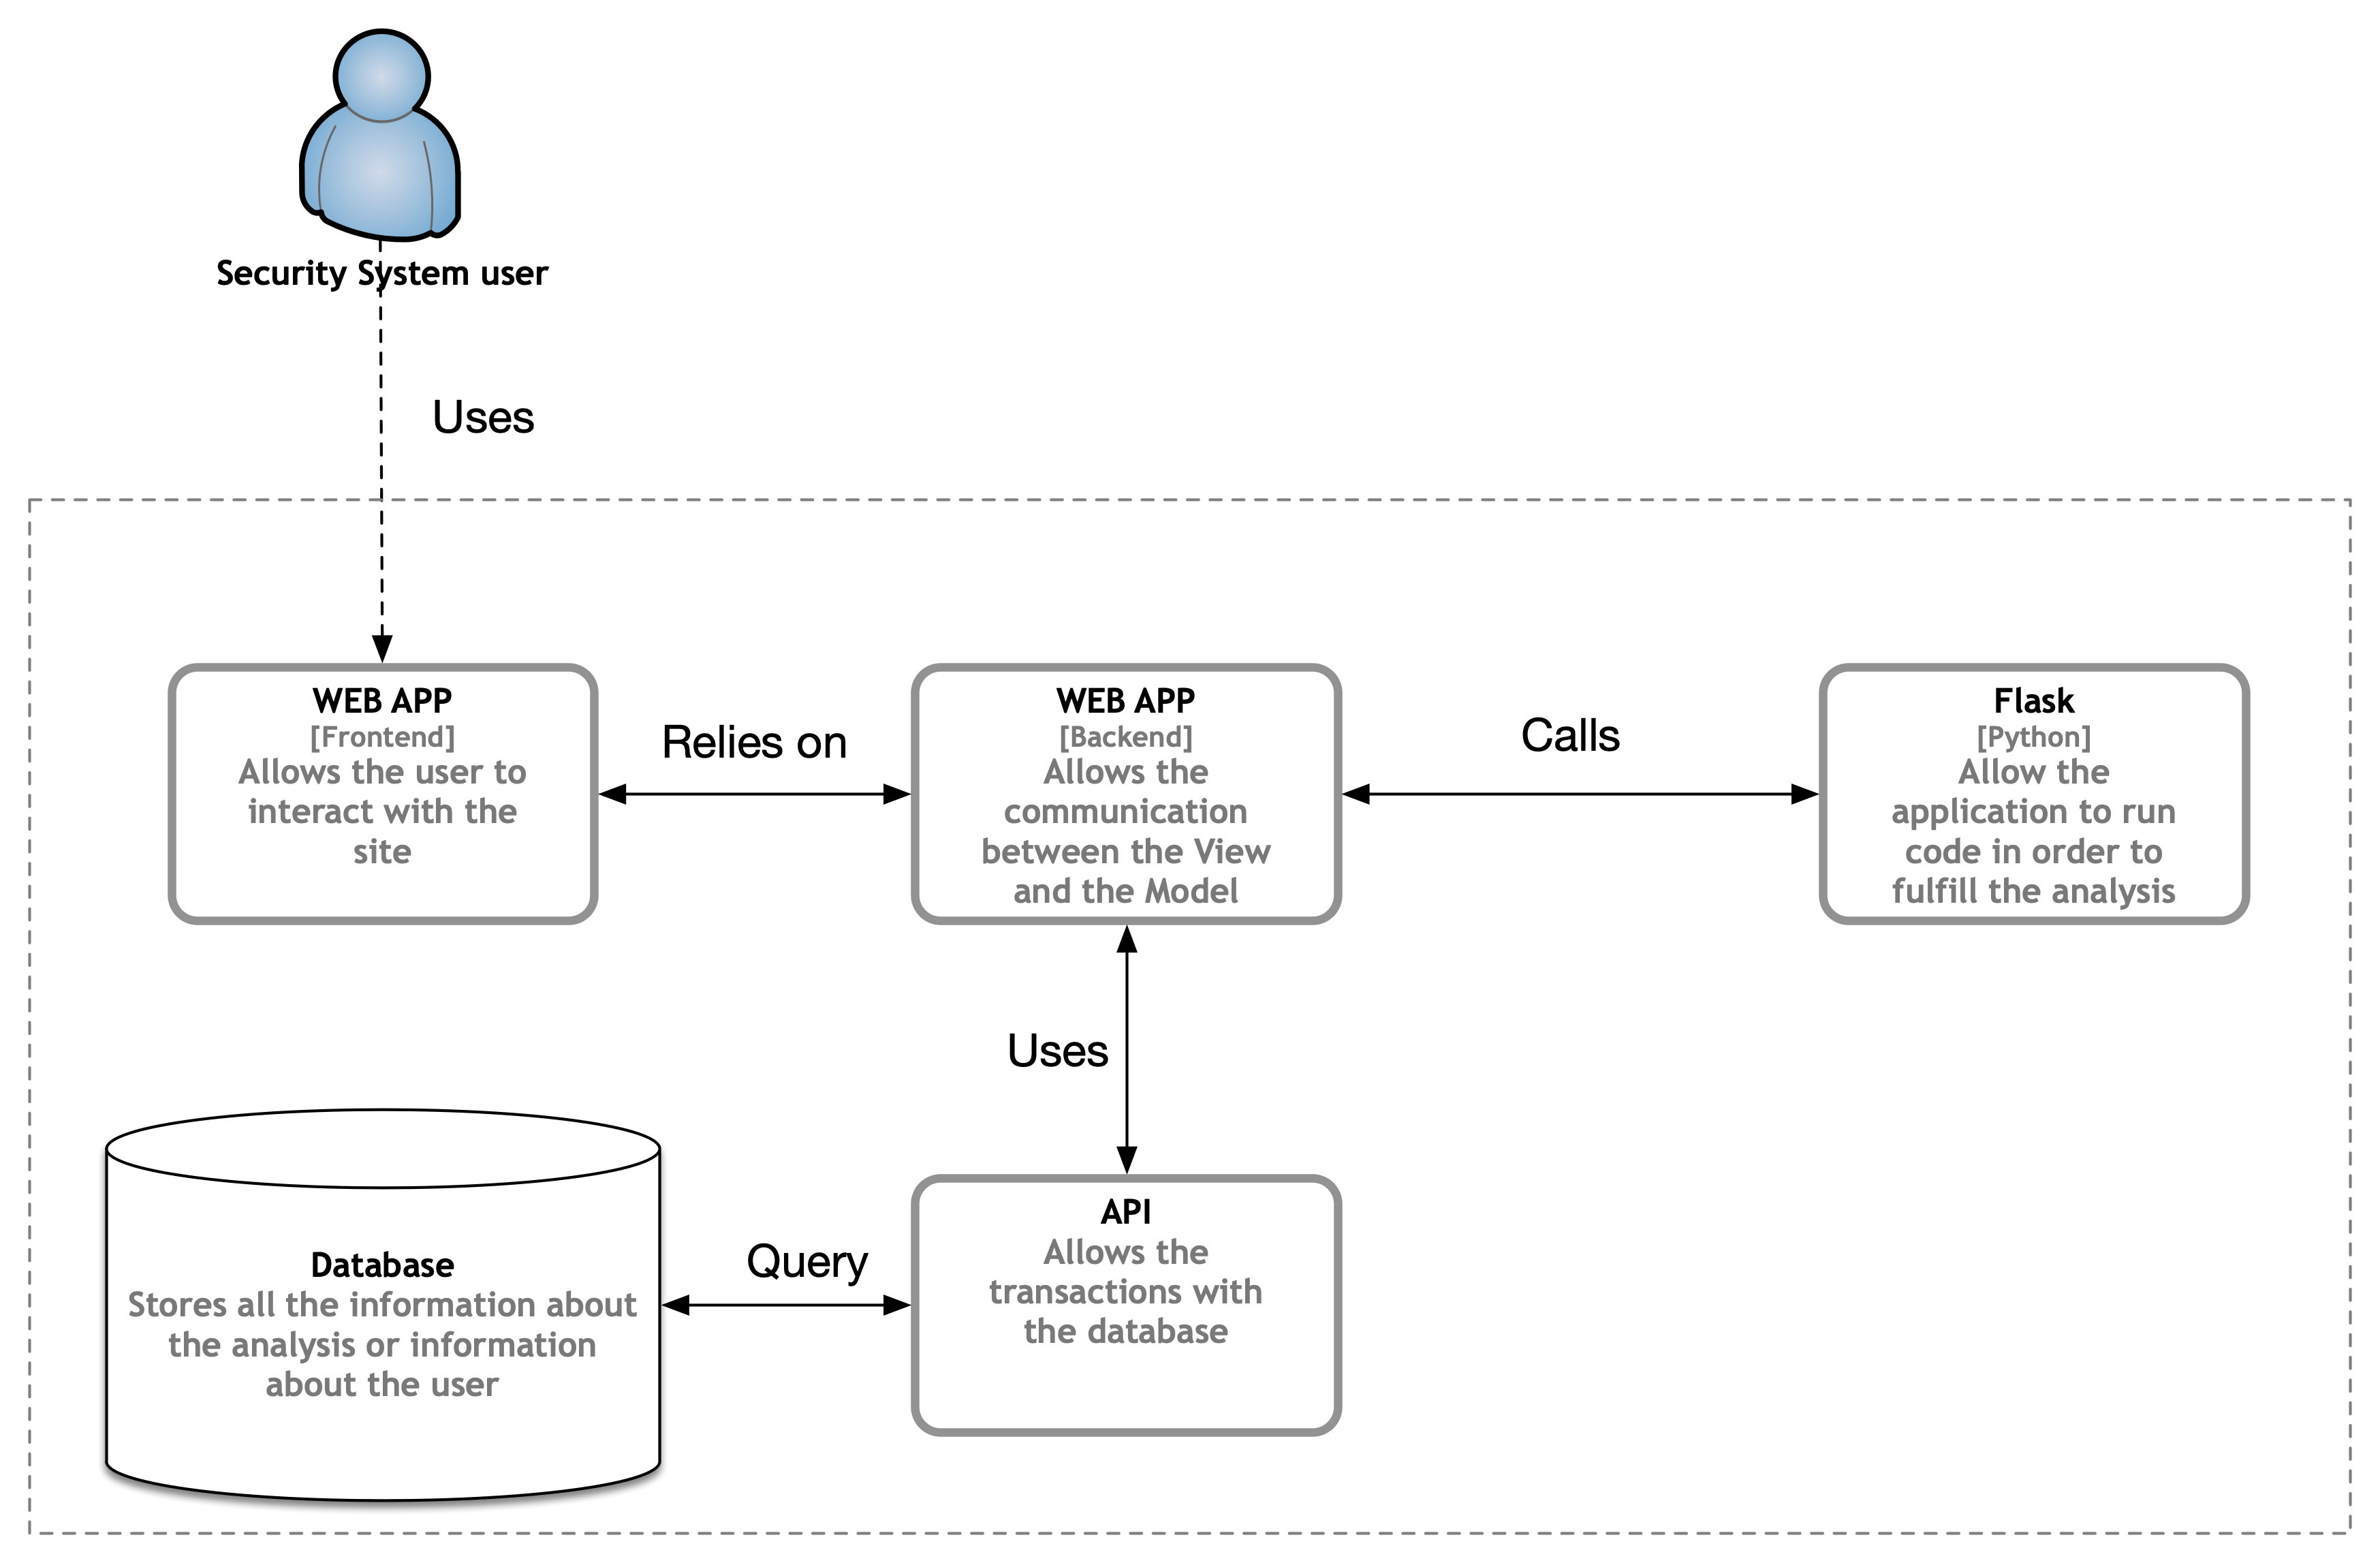
\includegraphics[width=14cm]{img/C42.jpg}
    \caption{Container diagram}
    \label{fig:c42}
\end{figure}

\clearpage

Finally on the Component diagram we identify the major structural building blocks and their interactions, it shows the different components of the application, their responsibilities and the technology/implementation details.

\begin{figure}[h!]
    \centering
    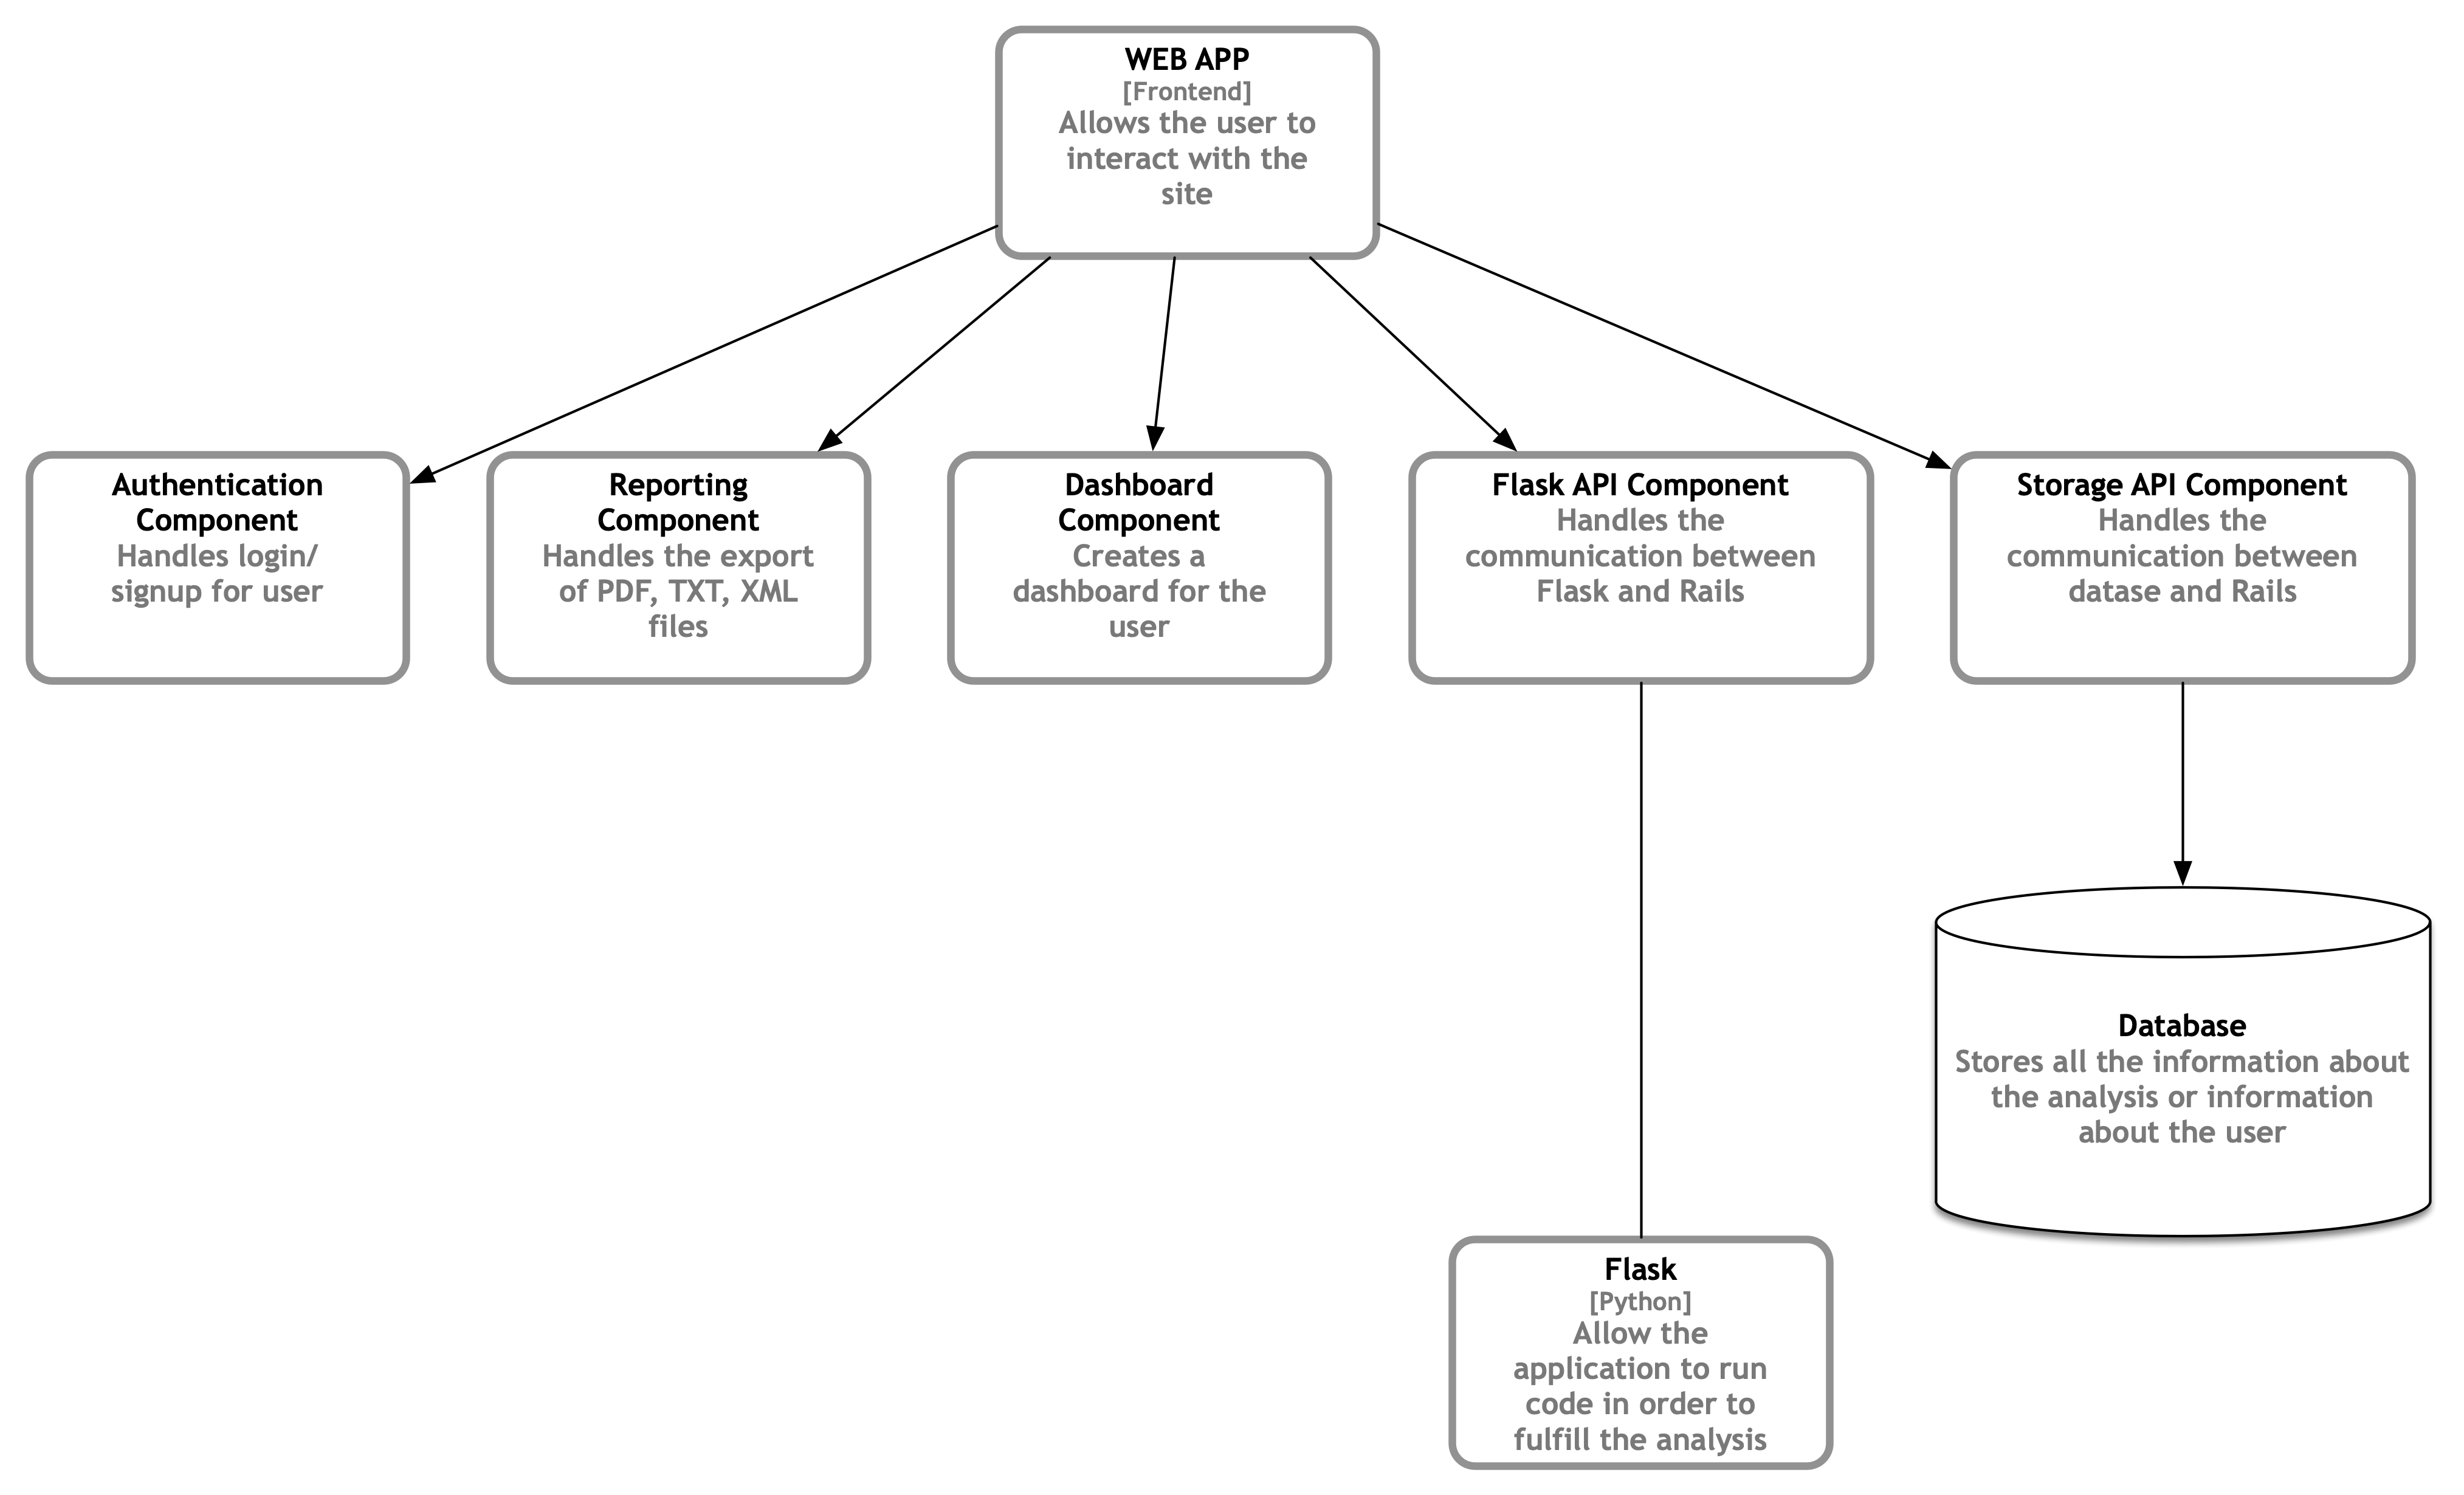
\includegraphics[width=14cm]{img/C43.jpg}
    \caption{Component diagram}
    \label{fig:c42}
\end{figure}
